% =============================================================================
% CalRank — Teaching Guide
% A ground-up explanation of the project, written so the reader can explain it
% to somebody else. Compile: tectonic TEACHING_GUIDE.tex
% =============================================================================
\documentclass[11pt,a4paper]{article}

\usepackage[utf8]{inputenc}
\usepackage[T1]{fontenc}
\usepackage[margin=1in]{geometry}
\usepackage{lmodern}
\usepackage{amsmath,amssymb}
\usepackage{graphicx}
\usepackage{booktabs}
\usepackage[table]{xcolor}
\usepackage{enumitem}
\usepackage{fancyhdr}
\usepackage[hidelinks]{hyperref}
\usepackage{microtype}
\usepackage{caption}

\graphicspath{{../data/figures/}}

\definecolor{headblue}{HTML}{2C3E6B}
\definecolor{rowlight}{HTML}{EAF0FA}
\definecolor{cleangreen}{HTML}{E6F5E8}
\definecolor{singleclasspink}{HTML}{FDE8E8}
\definecolor{keyyellow}{HTML}{FFF8E1}
\definecolor{keyborder}{HTML}{E6A700}
\definecolor{sayblue}{HTML}{EAF2FB}
\definecolor{sayborder}{HTML}{2C6FB5}
\newcommand{\thead}[1]{\textcolor{white}{\textbf{#1}}}

% --- Simple callout boxes (no exotic packages, guaranteed to compile) --------
\newcommand{\keybox}[2]{%
  \begin{center}
  \fcolorbox{keyborder}{keyyellow}{%
    \begin{minipage}{0.93\linewidth}
    \vspace{2pt}\textbf{#1}\\[2pt]#2\vspace{3pt}
    \end{minipage}}
  \end{center}}

\newcommand{\saybox}[1]{%
  \begin{center}
  \fcolorbox{sayborder}{sayblue}{%
    \begin{minipage}{0.93\linewidth}
    \vspace{2pt}\textbf{How to say it out loud}\\[3pt]\itshape #1\vspace{3pt}
    \end{minipage}}
  \end{center}}

\pagestyle{fancy}\fancyhf{}
\lhead{\small CalRank --- Teaching Guide}
\rhead{\small\thepage}
\renewcommand{\headrulewidth}{0.4pt}

\title{\bfseries CalRank: A Teaching Guide\\[4pt]
\large Everything in the project, from first principles,\\
so you can explain it to anybody}
\author{Prepared for Sayanjib Sur}
\date{}

\begin{document}
\maketitle
\thispagestyle{empty}

\begin{center}
\fcolorbox{black}{white}{\begin{minipage}{0.9\linewidth}
\vspace{4pt}
\textbf{How to use this document.} Part~I builds the background from zero: what a
re-ranker is, what calibration means, and how it is measured. Part~II describes what
we built. Part~III walks through every result with the exact numbers. Part~IV is the
part you will actually use when talking to someone: the pitch at three lengths, the
hard questions with answers, and the honest weaknesses. Part~V is a reference
appendix with every table and a glossary.

If you have ten minutes before a meeting, read Section~\ref{sec:pitch} and
Table~\ref{tab:allnumbers}.
\vspace{4pt}
\end{minipage}}
\end{center}

\tableofcontents
\newpage

% =============================================================================
\part{The Background}
% =============================================================================
\section{What problem does a re-ranker solve?}

Imagine a search engine with ten million documents. A user types a query. You cannot
run an expensive neural network on ten million documents in 200 milliseconds, so
real systems split the work into two stages.

\begin{enumerate}[leftmargin=*]
  \item \textbf{First stage (cheap, wide).} A fast method such as BM25 scans the
  whole collection and returns perhaps the top 100 candidates. BM25 counts word
  overlap between the query and each document, weighted so that rare words matter
  more. It is fast because it uses an inverted index, essentially a lookup table
  from words to documents. It is also fairly crude: it does not know that ``car''
  and ``automobile'' mean the same thing.

  \item \textbf{Second stage (expensive, narrow).} A neural \emph{re-ranker} reads
  those 100 candidates carefully and re-orders them. Because it only sees 100
  documents rather than ten million, you can afford a transformer.
\end{enumerate}

\subsection{Cross-encoders versus bi-encoders}
There are two ways to build the neural stage, and the difference matters.

A \textbf{bi-encoder} converts the query into a vector and each document into a
vector, separately, then compares the vectors with a dot product. Because documents
can be encoded in advance, this is fast. But the query and document never actually
``meet'' inside the network; they only interact through one number at the end.

A \textbf{cross-encoder} feeds the query and the document into the transformer
\emph{together}, as one concatenated input. Every word of the query can attend to
every word of the document. This captures much finer relationships, at the cost of
having to run the network once per query--document pair. That is exactly why it is
used in stage two and not stage one.

A cross-encoder outputs a single number, called a \textbf{logit}. Higher means more
relevant. Sort by it, and you have your ranking.

\keybox{The one-sentence version}{A cross-encoder re-ranker reads a query and a
document together and produces one number saying how relevant they are. Our project
is about whether that number can be trusted as a \emph{probability}, not just as a
sorting key.}

% =============================================================================
\section{From a score to a probability}

The raw logit can be any real number, say $-8.4$ or $+6.1$. To turn it into
something between 0 and 1, systems apply the \textbf{sigmoid} function:
\begin{equation}
\sigma(z) = \frac{1}{1 + e^{-z}}.
\end{equation}
So $\sigma(0) = 0.5$, $\sigma(2) \approx 0.88$, $\sigma(6) \approx 0.998$, and
$\sigma(-6) \approx 0.002$. Large positive logits get squashed towards 1, large
negative logits towards 0.

Now here is where the trouble starts. Because the output looks like a probability,
people \emph{use} it like one. Three real examples:

\begin{itemize}[leftmargin=*]
  \item \textbf{Retrieval-augmented generation (RAG).} A chatbot retrieves passages
  and feeds them to a language model. To avoid feeding it junk, the system keeps
  only passages scoring above, say, $0.7$ --- meaning ``at least 70\% likely
  relevant.''
  \item \textbf{Abstention.} A question-answering system refuses to answer when
  nothing retrieved looks confident enough, to avoid making things up.
  \item \textbf{Cascades.} If the small model is not confident, send the query to a
  bigger, costlier model.
\end{itemize}

In all three, somebody has assumed that $\sigma(\text{logit})$ equals
$P(\text{relevant} \mid \text{query}, \text{document})$.

\subsection{Why that assumption is not free}
Re-rankers are trained to get the \emph{order} right. The loss function rewards
putting relevant documents above non-relevant ones. It does not reward the numbers
being correct in an absolute sense.

Consider a model that outputs $0.99$ for every relevant document and $0.98$ for
every non-relevant one. Its ranking is \emph{perfect} --- every relevant document is
above every non-relevant one. But its probabilities are nonsense: it says ``98\%
confident'' about things that are not relevant at all.

\keybox{The core insight of the whole project}{Ranking well and being
probabilistically correct are two different skills. A model can be excellent at one
and terrible at the other. Nobody had systematically checked which situation we are
in for cross-encoder re-rankers. That is the gap we filled.}

% =============================================================================
\section{What ``calibration'' means}

A predictor is \textbf{calibrated} if its confidence matches reality. Formally: of
all the times it says ``70\%'', about 70\% should actually be correct.

\subsection{A worked example}
Suppose a model makes 100 predictions with confidence $0.9$. If it is calibrated,
roughly 90 of them are correct. If only 50 are correct, the model is
\textbf{overconfident} by 40 percentage points. If 99 are correct, it is
\textbf{underconfident}.

Overconfidence is the usual failure mode for neural networks, and it is what we
found here --- though, as we will see, not universally.

\subsection{Reliability diagrams}
The standard picture. Take all predictions, sort them into bins by confidence
($0$--$0.1$, $0.1$--$0.2$, and so on). For each bin, plot the average confidence on
the $x$-axis against the fraction actually correct on the $y$-axis.

A perfectly calibrated model traces the diagonal line $y = x$. Bars \emph{below} the
diagonal mean overconfidence (you claimed more than you delivered). Bars
\emph{above} mean underconfidence.

\subsection{Expected Calibration Error (ECE)}
ECE turns that picture into one number. With $B$ bins:
\begin{equation}
\mathrm{ECE} = \sum_{b=1}^{B} \frac{n_b}{N}\,
\bigl| \underbrace{\mathrm{acc}(b)}_{\text{fraction correct}} -
\underbrace{\mathrm{conf}(b)}_{\text{average confidence}} \bigr|
\end{equation}
In words: for each bin, measure the gap between claimed and actual, then average
those gaps weighted by how many predictions fall in each bin.

\textbf{Worked example.} Two bins. Bin~1 holds 80 predictions with average
confidence $0.9$, of which 40\% are correct. Bin~2 holds 20 predictions with average
confidence $0.6$, of which 60\% are correct.
\[
\mathrm{ECE} = \tfrac{80}{100}|0.4 - 0.9| + \tfrac{20}{100}|0.6 - 0.6|
             = 0.8 \times 0.5 + 0.2 \times 0 = 0.40
\]
An ECE of $0.40$ is very bad. For reference, a well-calibrated model scores below
$0.05$. \textbf{We measured raw ECE around $0.28$ on average.}

We used 15 equally-spaced bins throughout, and we tested whether that choice
mattered (Section~\ref{sec:robust}). It did not.

\subsection{The other two metrics}
\textbf{Maximum Calibration Error (MCE)} reports the single worst bin instead of the
average. Useful when you care about the worst case rather than the typical case.

\textbf{Brier score} is the mean squared error between the predicted probability and
the actual outcome (0 or 1):
$\mathrm{Brier} = \frac{1}{N}\sum_i (p_i - y_i)^2$. It is a \emph{proper scoring
rule}, meaning it rewards being both well-calibrated and discriminative at once.

\saybox{``Calibration means the number means what it says. If a re-ranker outputs
0.9, then out of a hundred such documents about ninety should really be relevant.
We measure the gap with Expected Calibration Error. Zero is perfect; anything above
0.05 is a problem. We found about 0.28.''}

% =============================================================================
\section{How you fix calibration: the three methods}

The good news is that you do not need to retrain anything. All three standard fixes
are \emph{post-hoc}: you take the trained model, hold out some labelled data, and
learn a small correction on top of its outputs.

\subsection{Temperature scaling (1 parameter)}
Divide the logit by a learned constant $T$ before the sigmoid:
\begin{equation}
p_{\text{calibrated}} = \sigma(z / T)
\end{equation}
When $T > 1$, this pulls all probabilities towards $0.5$, softening overconfidence.
When $T < 1$ it sharpens them. $T$ is found by minimising the negative
log-likelihood on the held-out set.

\textbf{Intuition:} it is a volume knob. It makes the model uniformly less shouty,
but it cannot change \emph{which} documents it shouts about.

\textbf{Crucially}, dividing every logit by the same positive number never changes
their order. So the ranking is untouched. This will matter a great deal later.

\subsection{Platt scaling (2 parameters)}
Fit a small logistic regression on the logit:
\begin{equation}
p_{\text{calibrated}} = \sigma(a z + b)
\end{equation}
The slope $a$ does what temperature does. The new part is the intercept $b$, which
\emph{shifts} the whole curve left or right.

\textbf{Intuition:} temperature can turn the volume down; Platt can also move where
the decision boundary sits. If a model's logits are systematically offset --- say
everything is shifted two units too high --- temperature cannot fix that, but Platt
can. This single extra parameter turns out to matter enormously.

Still monotone, so the ranking is still untouched.

\subsection{Isotonic regression (non-parametric)}
Learn an arbitrary increasing step function mapping raw probabilities to corrected
ones, using the pool-adjacent-violators algorithm. It can fit any monotone shape.

\textbf{Intuition:} maximum flexibility. The risk is overfitting --- with few
calibration examples it can memorise noise. Still monotone, so the ranking survives.

\keybox{All three preserve the ranking}{Every method here is \emph{monotone}: if
document A scored above document B before, it still does after. Calibration cannot
break your search results. This is why we can honestly say calibration is free.
(It also has a consequence we discovered later --- see
Section~\ref{sec:threshold}.)}

% =============================================================================
\part{What We Built}
% =============================================================================
\section{The experimental setup}

\subsection{Models: seven cross-encoders}
Chosen to span both size and training data. See Table~\ref{tab:models}.

\begin{table}[h]
\centering
\caption{The seven re-rankers studied.}\label{tab:models}
\small
\begin{tabular}{llrl}
\toprule
\rowcolor{headblue}
\thead{Name} & \thead{HuggingFace ID} & \thead{Params} & \thead{Notes} \\
\midrule
\rowcolor{rowlight}
TinyBERT-L2  & cross-encoder/ms-marco-TinyBERT-L-2-v2 & 4M   & tiny, distilled \\
MiniLM-L6    & cross-encoder/ms-marco-MiniLM-L-6-v2   & 22M  & \textbf{LangChain default} \\
\rowcolor{rowlight}
MiniLM-L12   & cross-encoder/ms-marco-MiniLM-L-12-v2  & 33M  & \textbf{Haystack default} \\
ELECTRA-base & cross-encoder/ms-marco-electra-base    & 110M & different pretraining \\
\rowcolor{cleangreen}
mxbai-base   & mixedbread-ai/mxbai-rerank-base-v1     & 184M & \textbf{not MS MARCO} \\
BGE-base     & BAAI/bge-reranker-base                 & 278M & multilingual backbone \\
\rowcolor{cleangreen}
BGE-large    & BAAI/bge-reranker-large                & 560M & largest \\
\bottomrule
\end{tabular}
\end{table}

The green rows were added later specifically to answer two anticipated criticisms:
``all your models are small'' and ``all your models are trained on the same data.''

\textbf{Why this matters practically:} MiniLM-L6 and MiniLM-L12 are the \emph{default}
re-rankers in LangChain, LlamaIndex, and Haystack. Thousands of production RAG
systems are running these right now, with no calibration step.

\subsection{Collections: eleven, of which five are usable}
Nine come from BEIR (a standard IR benchmark suite) and two from the TREC Deep
Learning track. The critical property is \textbf{prevalence}: the fraction of judged
query--document pairs that are actually relevant.

\begin{table}[h]
\centering
\caption{The eleven collections, ordered by prevalence. Green passes our validity
check; pink fails.}\label{tab:collections}
\small
\begin{tabular}{lrrrl}
\toprule
\rowcolor{headblue}
\thead{Collection} & \thead{Judged pairs} & \thead{Prevalence} & \thead{Negatives} & \thead{Domain} \\
\midrule
\rowcolor{cleangreen}
trec-dl-2020     & 5{,}686 & 0.17 & 4{,}727 & web passages \\
\rowcolor{cleangreen}
dbpedia-entity   & 9{,}182 & 0.35 & 5{,}996 & entity search \\
\rowcolor{cleangreen}
trec-dl-2019     & 4{,}612 & 0.35 & 3{,}000 & web passages \\
\rowcolor{cleangreen}
trec-covid       & 3{,}475 & 0.62 & 1{,}306 & biomedical \\
\rowcolor{cleangreen}
webis-touche2020 & 635     & 0.78 & 140     & argument retrieval \\
\rowcolor{singleclasspink}
scidocs          & 1{,}774 & 0.95 & 91      & citation prediction \\
\rowcolor{singleclasspink}
arguana          & 1{,}316 & 1.00 & 0       & counter-arguments \\
\rowcolor{singleclasspink}
fiqa             & 756     & 1.00 & 0       & financial QA \\
\rowcolor{singleclasspink}
nfcorpus         & 1{,}941 & 1.00 & 0       & health \\
\rowcolor{singleclasspink}
quora            & 1{,}278 & 1.00 & 0       & duplicate questions \\
\rowcolor{singleclasspink}
scifact          & 298     & 1.00 & 0       & scientific claims \\
\bottomrule
\end{tabular}
\end{table}

Look hard at that ``Negatives'' column. Six collections have almost none. This is not
a detail; it is the second half of the paper, and Section~\ref{sec:hazard} explains
why.

\subsection{The pipeline}
For each query: retrieve the BM25 top 100, score every pair with every model, and
record three things per pair --- the raw logit, its sigmoid, and the relevance label
from the human judgments ($-1$ if never judged, $0$ if judged non-relevant, $1$ if
judged relevant).

That produced roughly half a million scored pairs, of which about twenty thousand per
model are judged. Everything ran on a MacBook Air M4 using the Metal backend. No
cluster, no GPU rental.

\subsection{The protocol that keeps us honest}
For each model--collection pair, split the judged data 50/50, stratified by label,
with a fixed random seed of 42. Fit the calibrators on one half; measure on the
other half. \textbf{No calibrator is ever evaluated on the data it was fitted to.}

This matters most for isotonic regression, which is flexible enough to memorise its
training data and report a fake-perfect score if you let it.

\saybox{``We took seven re-rankers and eleven test collections, scored about half a
million query--document pairs, and measured how far their confidence was from
reality. Everything ran on a laptop, and every calibrator is tested on data it never
saw during fitting.''}

% =============================================================================
\part{The Results}
% =============================================================================
\section{Result 1: Re-rankers are overconfident --- mostly}

\subsection{The headline}
On the five collections where the measurement is valid, across the five original
models (25 model--collection pairs):

\begin{center}
\begin{tabular}{lr}
\toprule
Mean raw ECE & \textbf{0.280} \\
Typical optimal temperature $T$ & \textbf{3 to 12} \\
Pairs that are overconfident & \textbf{20 of 25} \\
\bottomrule
\end{tabular}
\end{center}

An ECE of $0.28$ means that on average, confidence and reality differ by 28
percentage points. A temperature of 8 means you must divide the logit by \emph{eight}
before the sigmoid produces anything sensible.

Figure~\ref{fig:heatmap} shows the whole picture at once: warm colours are bad, and
they dominate.

\begin{figure}[h]
\centering
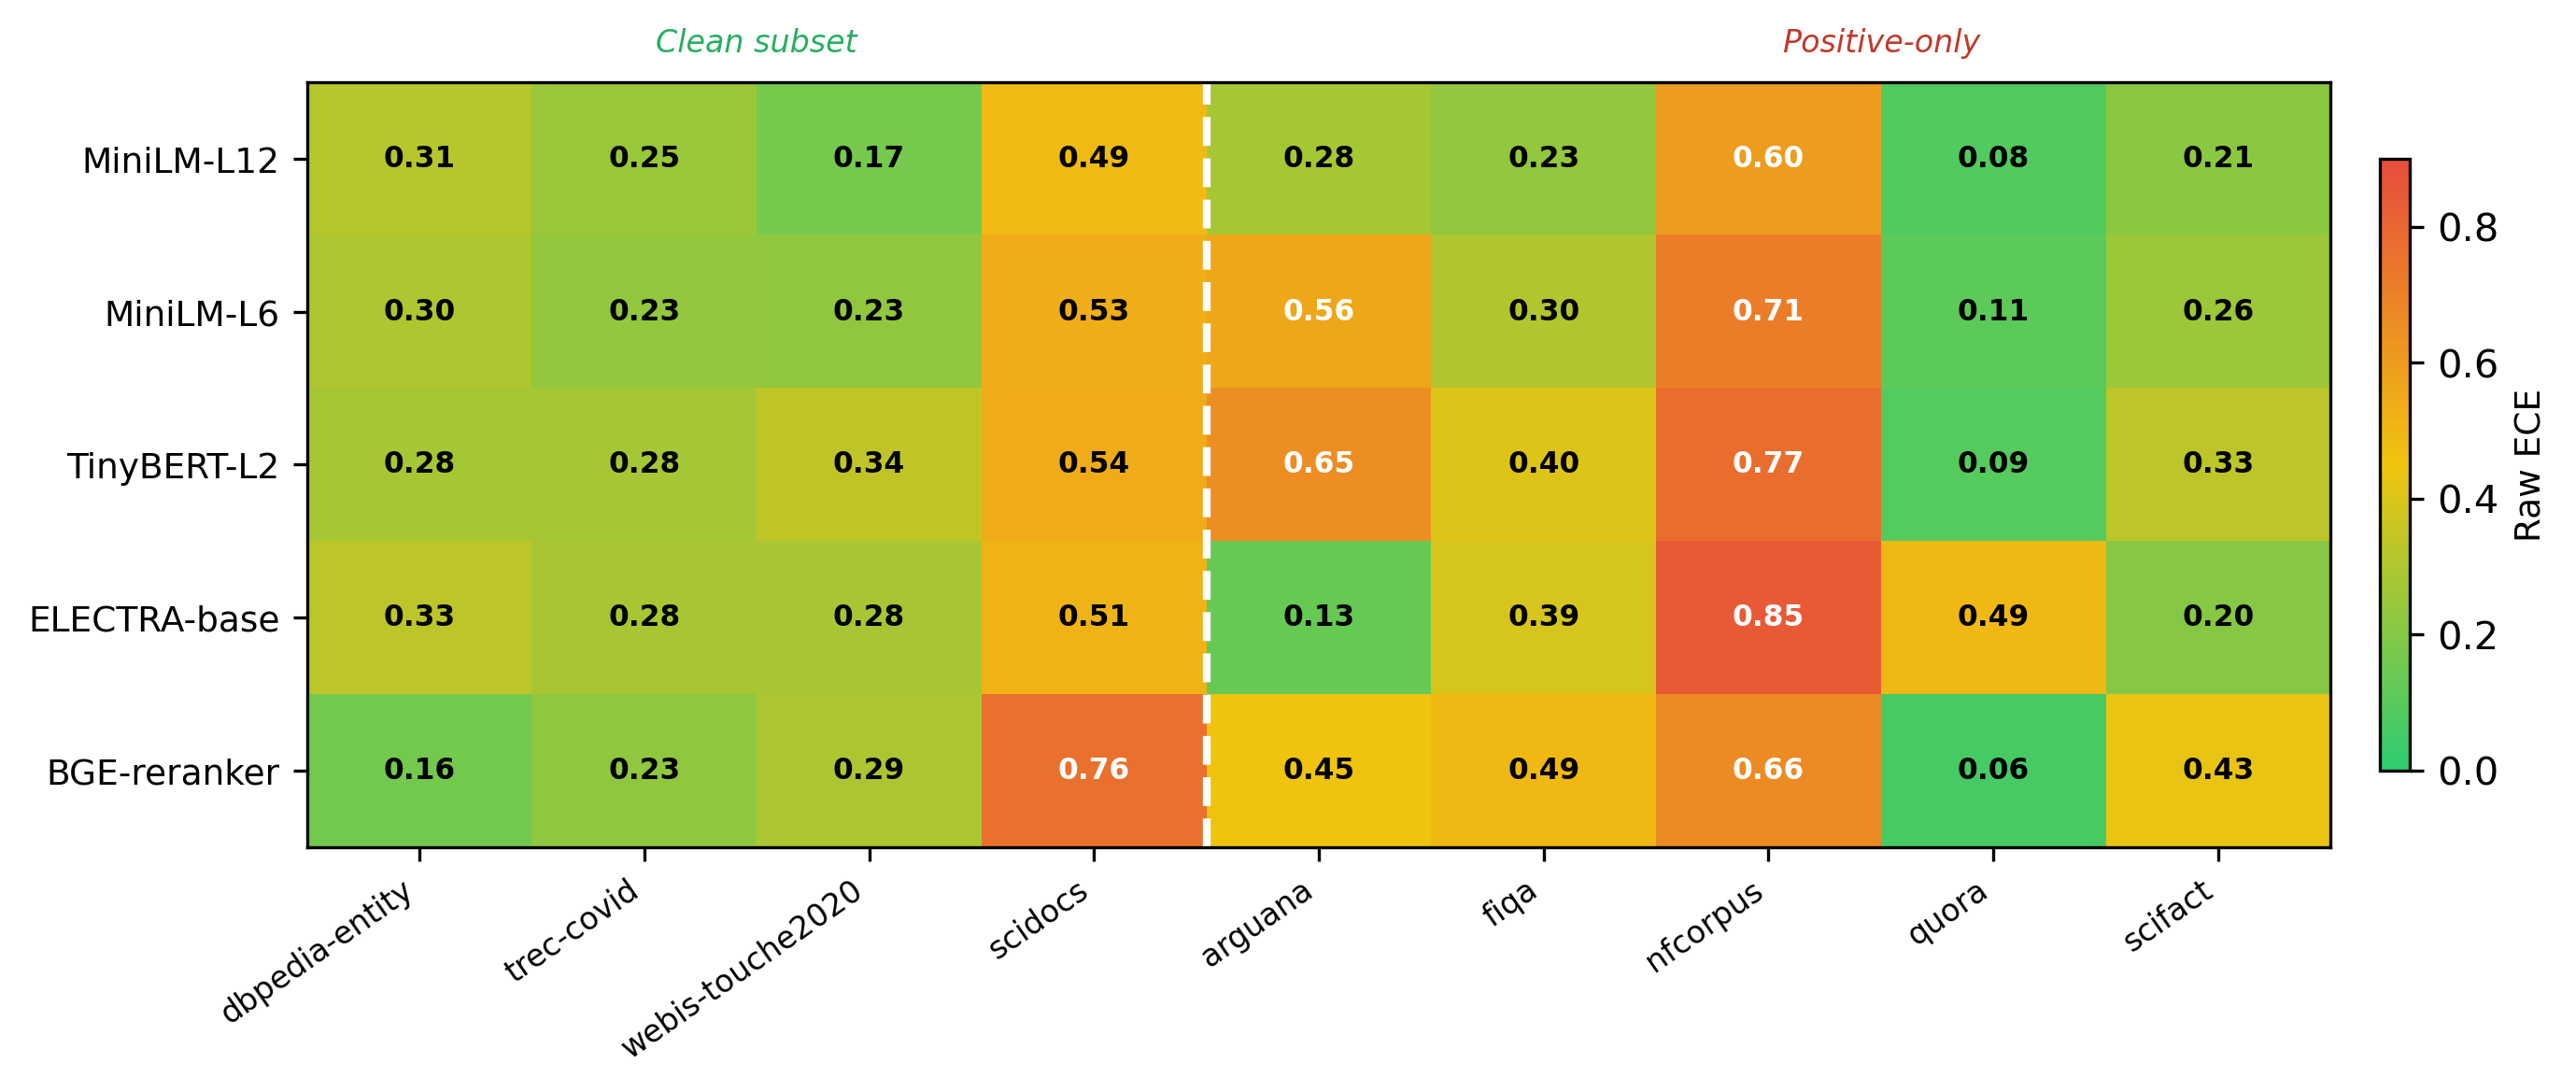
\includegraphics[width=\textwidth]{paper_fig_ece_heatmap.png}
\caption{Raw ECE for every model on every collection. Green is well calibrated, red
is badly calibrated.}\label{fig:heatmap}
\end{figure}

\subsection{The honest qualification}
Our first draft said ``every model is severely overconfident.'' When we added the
TREC DL collections, that turned out to be too strong, and we corrected it.

Because ECE uses an absolute value, it tells you the \emph{size} of the error but not
its \emph{direction}. So we computed a signed version. Result: 20 of 25 pairs are
overconfident (mean signed error $+0.139$), but on \textbf{webis-touche2020} four of
five models are actually \emph{under}-confident (mean $-0.114$).

There is a pattern, and it makes sense. The worst overconfidence is on trec-dl-2020,
which has the \emph{lowest} prevalence ($0.17$). These models were trained on MS
MARCO, where nearly every candidate shown during training was relevant. They
inherited a prior that says ``most things are relevant.'' Show them a collection
where only 17\% are relevant and they are wildly overconfident. Show them
webis-touche, where 78\% are relevant, and they undershoot.

\keybox{Why we kept this in}{We could have quietly dropped the exception. Reporting
it makes the paper more credible, not less --- and it produced a genuine explanation
(training-set prevalence) that a cleaner story would have hidden.}

% =============================================================================
\section{Result 2: The methodological hazard}\label{sec:hazard}

This is the most important part of the project, and the part that makes it more than
a measurement exercise.

\subsection{The setup}
Six of our eleven collections have almost no negative judgments. Five have
\emph{exactly zero} --- every single judged document is relevant.

Why? Because of how these collections were built. Human assessors were shown
documents and asked to mark the relevant ones. Documents they did not mark were left
\emph{unjudged}, not marked as non-relevant. So the judged set is all positive.

\subsection{What goes wrong}
Ask yourself: what does calibration even mean when every label is 1?

A calibrator that simply outputs ``1.0'' for everything is now \emph{perfect}. Its
confidence (1.0) exactly matches reality (100\% of labels are 1). ECE $= 0$.

That is not calibration. That is a degenerate answer to a degenerate question.

And that is exactly what isotonic regression does. On these collections it learns to
map everything to the majority class and scores \textbf{ECE = 0.000}. If you did not
know where that number came from, you would think isotonic regression was miraculous.

Meanwhile temperature scaling \emph{fails} on these collections --- sometimes it makes
ECE worse. Why? The optimiser is trying to minimise loss with no negative examples to
learn from. There is no signal telling it to reduce confidence. When we removed the
search cap, the temperature diverged to infinity, which collapses every probability
towards $0.5$. That is the best it can do when the labels are all positive but many
logits are negative.

\begin{figure}[h]
\centering
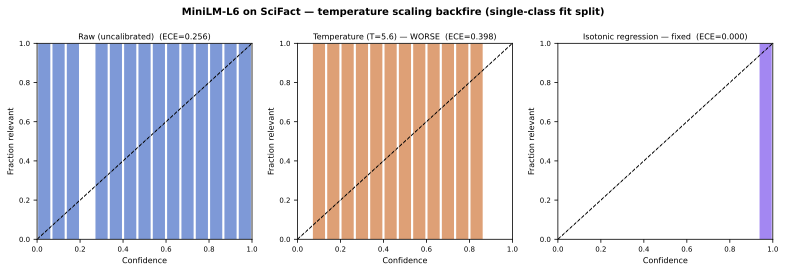
\includegraphics[width=0.8\textwidth]{paper_fig2_minilm_scifact_temp_backfire.png}
\caption{MiniLM-L6 on scifact (prevalence 1.0). Temperature scaling makes calibration
\emph{worse}; isotonic regression scores a fake-perfect zero. Neither number means
anything.}\label{fig:backfire}
\end{figure}

\subsection{The trap}
Here is what happens if you do the obvious thing and pool all the data:

\begin{center}
\begin{tabular}{lr}
\toprule
Temperature scaling improves ECE in & 27 of 45 pairs (Wilcoxon $p = 0.024$) \\
Isotonic regression improves ECE in & 45 of 45 pairs \\
\bottomrule
\end{tabular}
\end{center}

The natural conclusion --- ``temperature scaling is unreliable, isotonic regression is
excellent'' --- is \textbf{wrong in both halves}. It is an artifact of including
collections where the measurement is meaningless.

\keybox{Why this is a real contribution}{A statistically significant result, computed
correctly, that leads to the wrong engineering decision. Anyone measuring calibration
on BEIR without checking prevalence would fall into this. We fell into it ourselves
first --- that is how we found it.}

\subsection{Is this just the ``incomplete judgments'' problem?}
This is the question a knowledgeable IR person will ask, so know the answer cold.

The classic problem (Buckley \& Voorhees, 2004) is about \emph{unjudged} documents
distorting ranking metrics like nDCG. The standard fix is to evaluate only on judged
documents --- that is what bpref and condensed lists do.

\textbf{Our problem survives that fix.} We already evaluate on judged pairs only. The
degeneracy happens \emph{inside} the judged set, because of its class balance. Three
differences:

\begin{enumerate}[leftmargin=*]
  \item \textbf{Their concern:} missing documents outside the pool.
  \textbf{Ours:} label imbalance inside it.
  \item \textbf{Their fix} (judged-only evaluation) \textbf{is our starting
  condition.} It does not help.
  \item \textbf{Their consequence:} a metric value is biased. \textbf{Ours:} the
  \emph{ranking of methods} inverts --- the trivial method wins.
\end{enumerate}

\saybox{``Incomplete judgments is a known problem about unjudged documents biasing
ranking metrics, and the standard fix is to evaluate only on judged documents. Our
problem is different because it \emph{survives} that fix --- it happens inside the
judged set, and it doesn't just bias a number, it flips which method looks best.''}

% =============================================================================
\section{Result 3: The diagnostic (our tool)}\label{sec:diagnostic}

Noticing a problem is worth something. Giving people a check they can run is worth
more. So we turned the observation into a rule, fixed \emph{before} looking at any
results:

\begin{equation}
\text{Valid} \iff \min(n_+, n_-) \geq 100 \quad\text{and}\quad \pi \leq 0.90
\end{equation}
where $n_+$ and $n_-$ are the counts of positive and negative judged pairs, and
$\pi$ is the prevalence.

\textbf{In words:} you need at least 100 examples of the rarer class, and the data
must not be more than 90\% one class.

\subsection{What it caught}
Applied to all eleven collections, it flags six. Five are the obvious positive-only
ones. The sixth is the interesting one: \textbf{scidocs}, which has prevalence $0.95$
and only \textbf{91 negative judgments}.

We had been treating scidocs as a ``clean'' collection. The diagnostic said no.

\subsection{Why we believe the diagnostic works}
Two completely independent pieces of evidence, neither of which we were looking for,
agree that scidocs is broken:

\begin{enumerate}[leftmargin=*]
  \item When we removed the temperature search cap, scidocs' fitted temperature
  \textbf{diverged to infinity} --- behaviour otherwise seen only on the
  positive-only collections.
  \item In the transfer experiment, scidocs was the \textbf{only} supposedly-clean
  collection whose behaviour did not match its neighbours.
\end{enumerate}

\keybox{The strongest argument in the paper}{A rule we fixed in advance, plus two
unrelated empirical symptoms, all point at the same collection. That is much harder
to dismiss than any one of them alone.}

Acting on our own diagnostic, we then went looking for collections that would
\emph{pass} it. That is why we added TREC Deep Learning 2019 and 2020, which are
pooled far more deeply and supply 3{,}000 and 4{,}727 negatives respectively. That
took the usable set from three collections to five.

% =============================================================================
\section{Result 4: When measurement is valid, everything works}

On the five valid collections, all three methods improve calibration, in a consistent
order.

\begin{table}[h]
\centering
\caption{Mean ECE on the core subset, five original models, 25 pairs.}
\small
\begin{tabular}{lrl}
\toprule
\rowcolor{headblue}
\thead{Method} & \thead{Mean ECE} & \thead{Reading} \\
\midrule
\rowcolor{rowlight}
Uncalibrated         & 0.280 & badly wrong \\
Temperature scaling  & 0.177 & clear improvement \\
\rowcolor{rowlight}
Platt scaling        & 0.046 & very good \\
Isotonic regression  & \textbf{0.029} & best \\
\bottomrule
\end{tabular}
\end{table}

All six pairwise comparisons survive \textbf{Holm--Bonferroni correction} (the
largest adjusted $p$-value is $1.05 \times 10^{-4}$). We apply that correction
because running six tests on the same data inflates the chance of a false positive;
Holm controls for it.

\subsection{The prevalence effect}
Look at how the gap between temperature and Platt depends on prevalence:

\begin{table}[h]
\centering
\caption{Mean ECE by collection. Temperature struggles most where prevalence is
furthest from balance.}
\small
\begin{tabular}{lrrrrr}
\toprule
\rowcolor{headblue}
\thead{Collection} & \thead{Prev.} & \thead{raw} & \thead{temp} & \thead{Platt} & \thead{iso} \\
\midrule
\rowcolor{cleangreen}
trec-dl-2020     & 0.17 & 0.324 & 0.284 & 0.021 & 0.016 \\
dbpedia-entity   & 0.35 & 0.276 & 0.182 & 0.030 & 0.022 \\
\rowcolor{cleangreen}
trec-dl-2019     & 0.35 & 0.285 & 0.146 & 0.043 & 0.039 \\
trec-covid       & 0.62 & 0.255 & 0.056 & 0.054 & 0.031 \\
\rowcolor{cleangreen}
webis-touche2020 & 0.78 & 0.262 & 0.221 & 0.082 & 0.038 \\
\bottomrule
\end{tabular}
\end{table}

On trec-covid (prevalence $0.62$, near balance) temperature and Platt are
indistinguishable: $0.056$ versus $0.054$. On trec-dl-2020 (prevalence $0.17$)
temperature manages only $0.284$ while Platt reaches $0.021$ --- a 13-fold difference.

\textbf{This is the intercept doing its work.} Temperature can only rescale. When the
class balance is far from the point where the sigmoid is centred, you need to
\emph{shift}, and only Platt and isotonic can shift.

\begin{figure}[h]
\centering
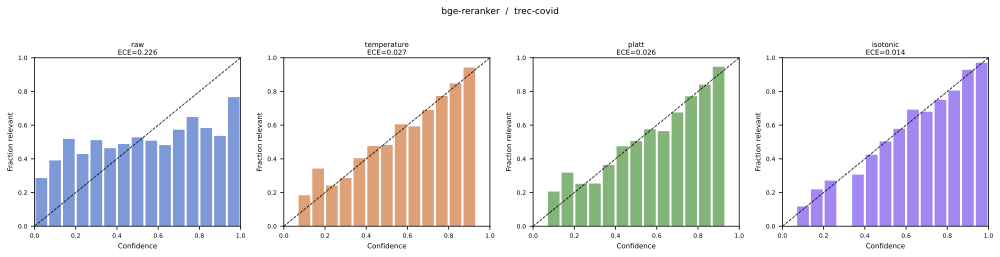
\includegraphics[width=0.95\textwidth]{paper_fig_bge_treccovid_4panel.png}
\caption{BGE on trec-covid: raw, then temperature, Platt, isotonic. The bars move
from well below the diagonal up onto it.}\label{fig:fourpanel}
\end{figure}

% =============================================================================
\section{Result 5: The advice reverses in deployment}

Here is a result we did not expect, and it is the most practically useful thing in
the paper.

\subsection{The question}
Everything above assumes you have labelled data \emph{from your own domain} to fit
the calibrator on. In reality, if you deploy a re-ranker on a new corpus, you usually
have no relevance judgments for it at all.

So: can you fit a calibrator on domains you \emph{do} have, and reuse it?

We tested this by leave-one-domain-out --- fit on four collections, test on the fifth.

\subsection{The answer}
\begin{table}[h]
\centering
\caption{Calibrator transfer, core subset, 25 pairs. ``Retention'' is the fraction of
the in-domain benefit that survives transfer.}
\small
\begin{tabular}{lrrrr}
\toprule
\rowcolor{headblue}
\thead{Regime} & \thead{Temperature} & \thead{Platt} & \thead{Temp.\ retention} & \thead{Platt retention} \\
\midrule
\rowcolor{rowlight}
Uncalibrated       & \multicolumn{2}{c}{0.280} & --- & --- \\
Transferred        & 0.191 & 0.178 & \textbf{87\%} & \textbf{44\%} \\
\rowcolor{rowlight}
In-domain (best case) & 0.177 & 0.046 & 100\% & 100\% \\
\midrule
Std.\ dev.\ (transferred) & 0.090 & 0.122 & \multicolumn{2}{l}{lower = more reliable} \\
Beats doing nothing & 22/25 & 19/25 & \multicolumn{2}{l}{} \\
\bottomrule
\end{tabular}
\end{table}

\textbf{Temperature travels. Platt does not.} Temperature keeps 87\% of its value when
moved to an unseen domain. Platt keeps 44\%, is 36\% more variable, and on
webis-touche2020 it is \emph{worse than applying no calibration at all}, for every
single model.

\begin{figure}[h]
\centering
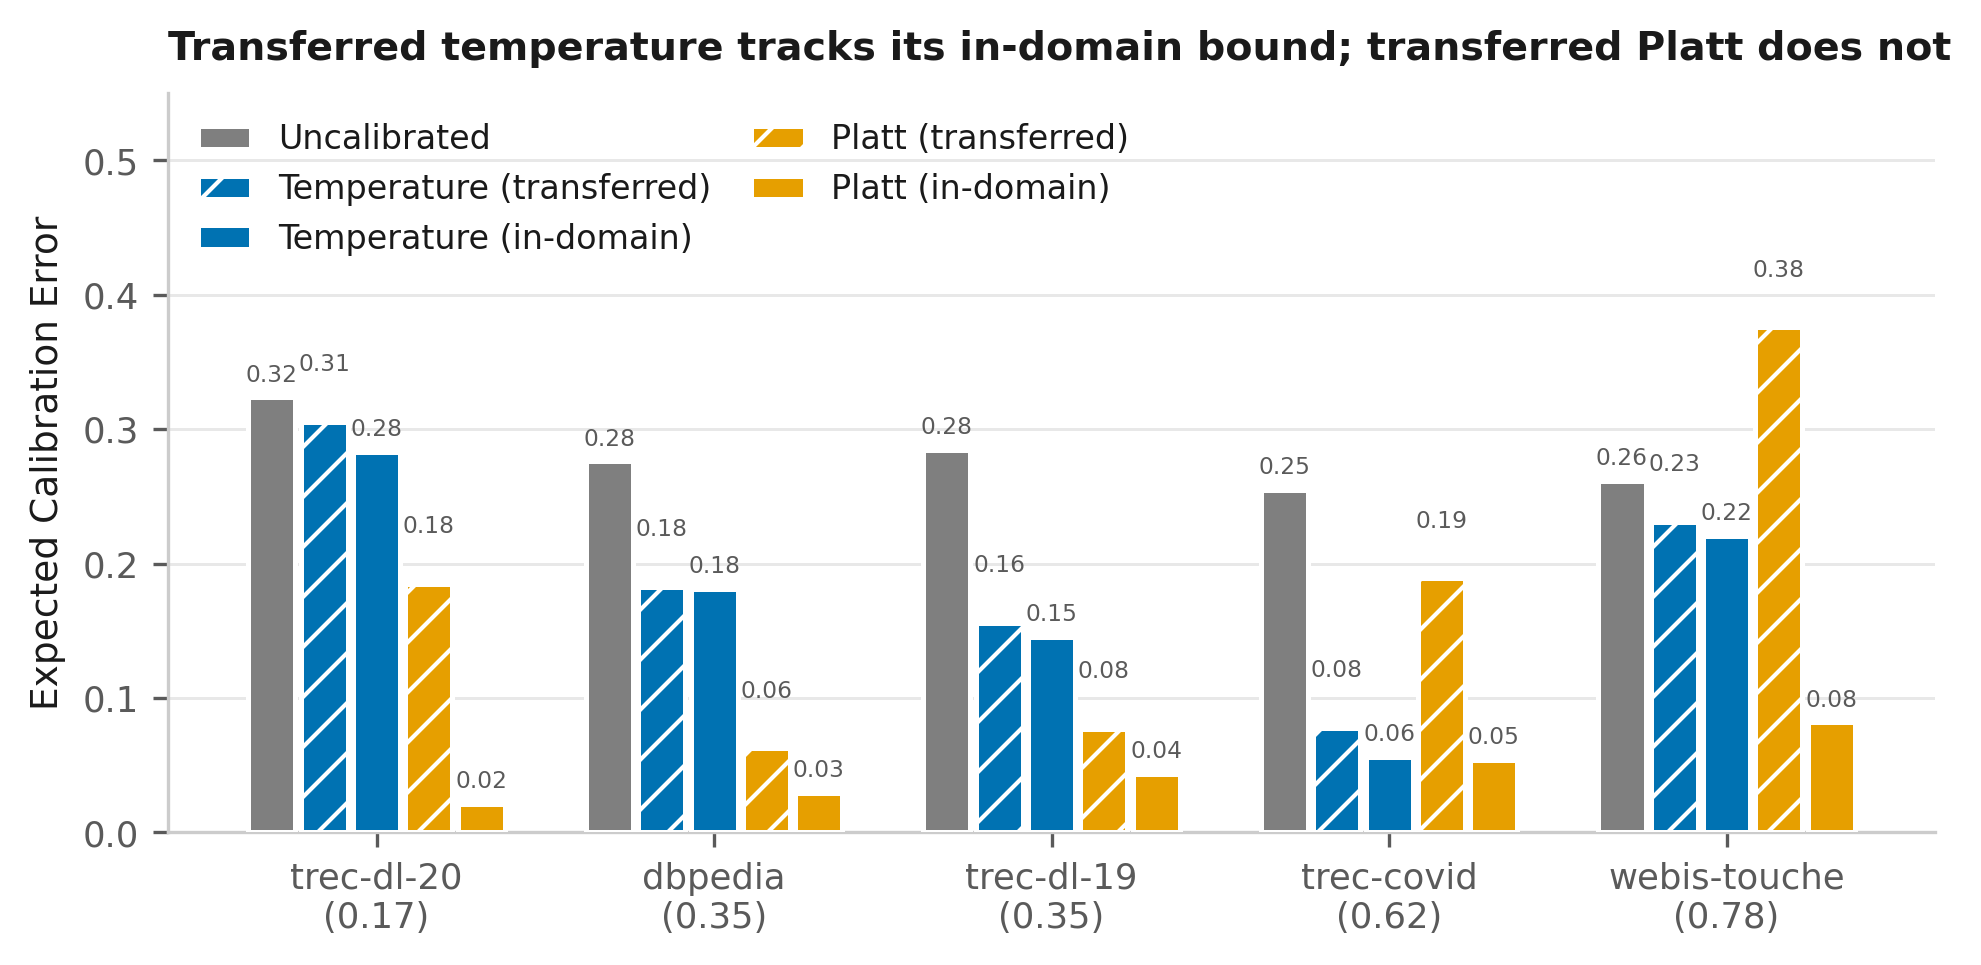
\includegraphics[width=\textwidth]{paper_fig_transfer.png}
\caption{Hatched bars are transferred calibrators; solid bars are in-domain. The blue
(temperature) pairs are nearly the same height. The orange (Platt) pairs are
not.}\label{fig:transfer}
\end{figure}

\subsection{Why}
It is the same intercept that made Platt good in the first place. An intercept
encodes \emph{where the decision boundary sits}, and that is a property of the
\emph{domain}, not of the model. Move it somewhere else and you import a bias.

A temperature encodes how \emph{sharp} the logit distribution is, which is a property
of the model and stays roughly constant. Our fitted temperatures vary only by a
factor of 1.7 to 2.9 across collections --- which is exactly why quoting one
temperature per model is defensible.

\keybox{The practical rule}{\textbf{If you have in-domain labelled data with
negatives:} use isotonic or Platt. \textbf{If you do not:} use temperature, and do
\emph{not} borrow a Platt calibrator from another domain. The best method in the lab
is nearly the worst in the field.}

% =============================================================================
\section{Result 6: What calibration actually buys you}\label{sec:threshold}

\subsection{First, what it does not buy}
Remember that all three methods are monotone --- they never change the order of
documents. That has a consequence we worked out and stated explicitly:

\keybox{Monotone calibration cannot improve the precision/coverage frontier}{If the
order never changes, then for any fixed number of accepted documents, the accepted
\emph{set} is identical before and after calibration --- and so is its precision.
Calibration cannot make a filtering system better at filtering. Full stop.}

We confirmed this empirically too: nDCG@10 changes by at most $1.0 \times 10^{-4}$
across all pairs. Ranking quality is untouched, for better or worse.

So if calibration cannot improve what the system achieves, what is it for?

\subsection{What it does buy: the threshold starts meaning something}
Imagine you are building a RAG system. You decide: ``only forward passages I believe
are at least 80\% likely relevant.'' You set the threshold to $0.8$. What precision
do you actually get?

\begin{table}[h]
\centering
\caption{Realised precision when the operator sets $\tau = 0.8$. The request is 0.80
in every row.}\label{tab:threshold}
\small
\begin{tabular}{lrrr}
\toprule
\rowcolor{headblue}
\thead{Collection} & \thead{Uncalibrated} & \thead{Temperature} & \thead{Isotonic} \\
\midrule
\rowcolor{cleangreen}
trec-dl-2020     & \textbf{0.357} & 0.646 & 0.812 \\
dbpedia-entity   & 0.542 & 0.890 & 0.867 \\
\rowcolor{cleangreen}
trec-dl-2019     & 0.553 & 0.765 & 0.789 \\
trec-covid       & 0.712 & 0.843 & 0.844 \\
\rowcolor{cleangreen}
webis-touche2020 & 0.854 & 0.783 & 0.851 \\
\midrule
\rowcolor{rowlight}
\textbf{Spread (max $-$ min)} & \textbf{0.497} & 0.243 & \textbf{0.078} \\
\textbf{Mean} & 0.603 & 0.785 & 0.833 \\
\bottomrule
\end{tabular}
\end{table}

Read the first column. You asked for 80\%. You received anywhere from \textbf{36\% to
85\%} depending on which collection you happened to deploy on. On trec-dl-2020 you got
\emph{less than half} of what you asked for. The same nominal setting denotes five
completely different operating points.

After isotonic calibration, the spread collapses from $0.497$ to $0.078$. The
threshold becomes portable.

\begin{figure}[h]
\centering
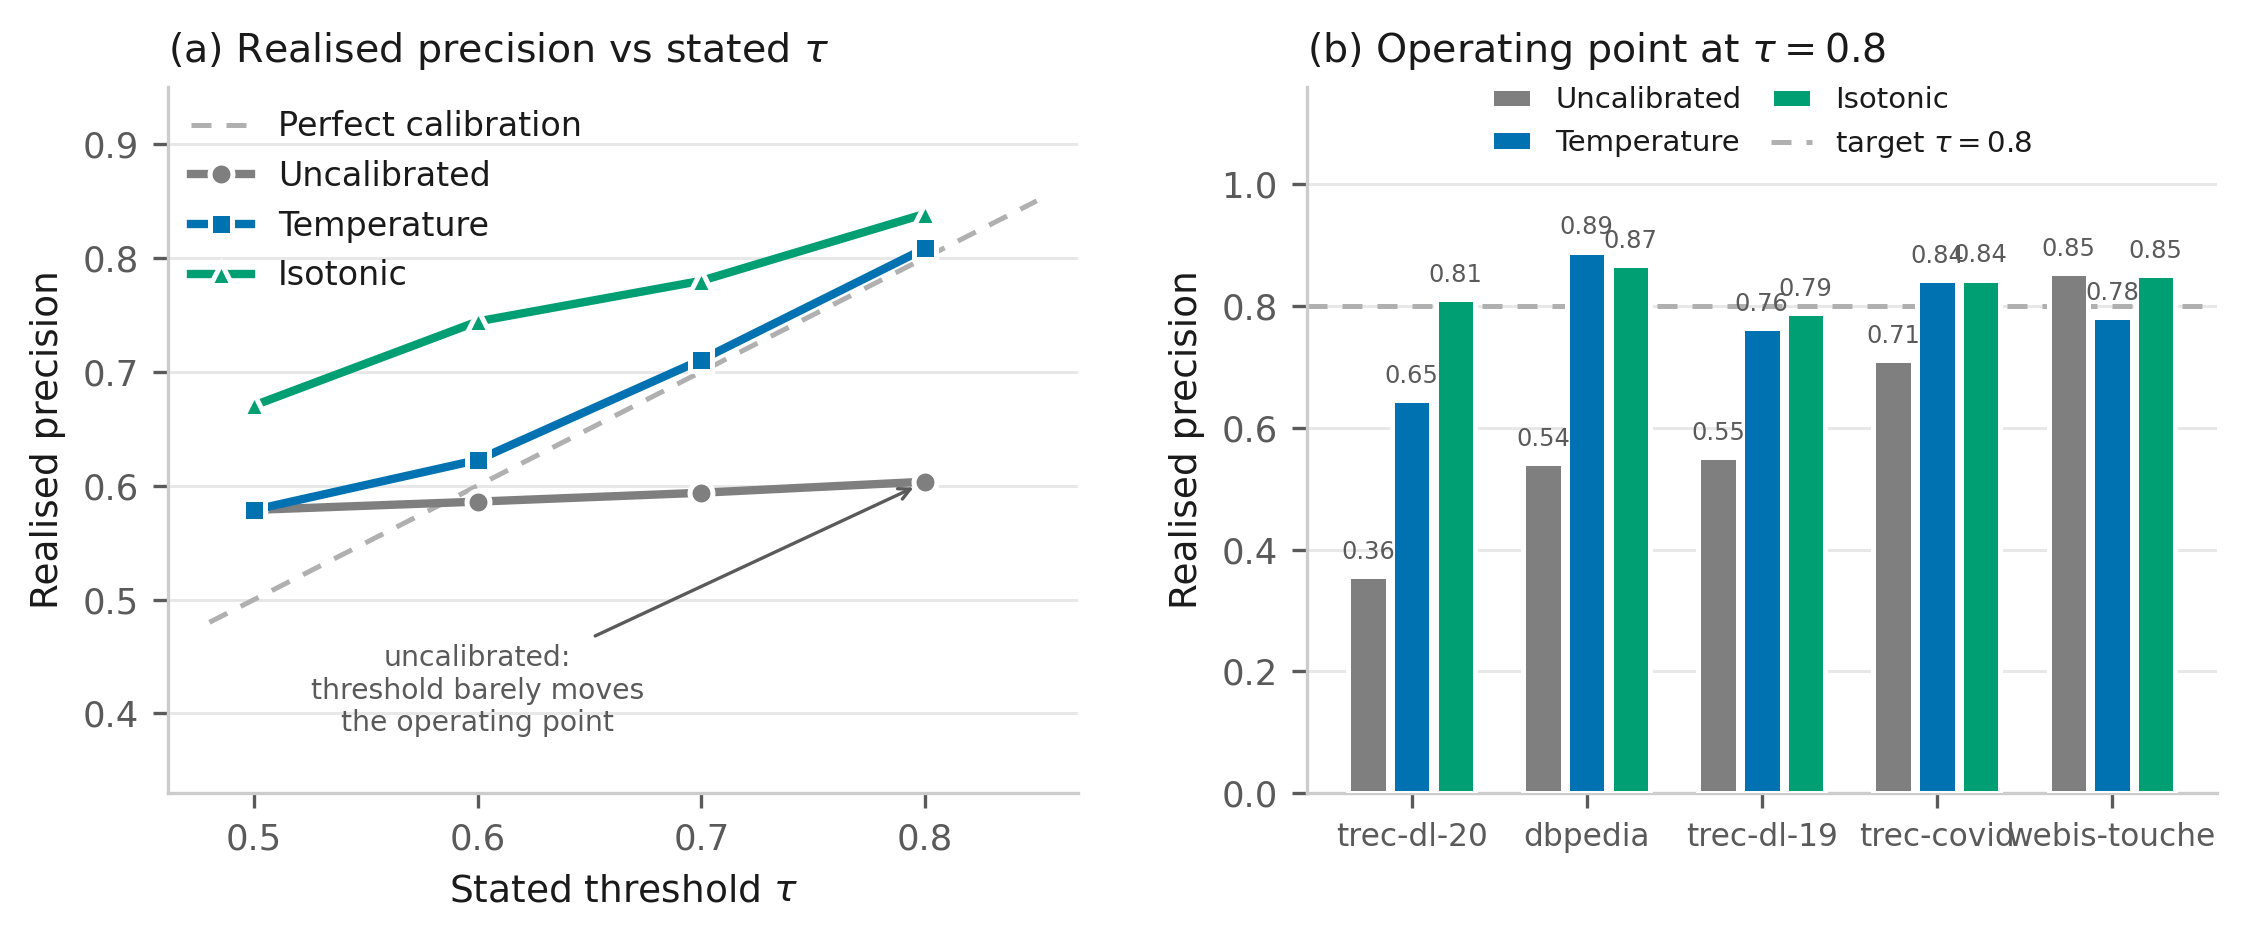
\includegraphics[width=\textwidth]{paper_fig_threshold_honesty.png}
\caption{(a) Raising the threshold barely moves the uncalibrated operating point ---
the dial is connected to nothing. (b) At $\tau=0.8$, uncalibrated precision varies
wildly across collections; after calibration it does not.}\label{fig:honesty}
\end{figure}

Panel (a) shows something else worth knowing. Raising $\tau$ from $0.5$ to $0.8$ moves
uncalibrated precision from $0.685$ to only $0.703$ --- under two points. The scores
are so compressed near 1.0 that the threshold selects almost the same set no matter
where you put it. The control does not control anything.

\saybox{``Calibration doesn't make the system better at finding relevant documents ---
it mathematically can't, because it never reorders anything. What it does is make the
threshold mean what it says. Before calibration, setting a threshold of 0.8 gave us
anywhere between 36\% and 85\% precision depending on the dataset. After, it's between
79\% and 87\%. That's the difference between a knob that works and a knob that
doesn't.''}

\subsection{One honest caveat}
Calibrated scores at $\tau = 0.8$ average $0.833$ --- slightly \emph{above} the
requested $0.80$. So they under-promise a little. That is the safer direction to err,
but it is not exact. Also, because calibration pushes probabilities down, a fixed
threshold accepts far fewer documents afterwards. Thresholds carried over from an
uncalibrated system need re-tuning.

% =============================================================================
\section{Result 7: Does model choice matter?}

We added two models specifically to widen the range: BGE-large (560M, the biggest)
and mxbai-base (184M, trained without MS MARCO).

\begin{table}[h]
\centering
\caption{All seven models on the core subset, ordered by size.}\label{tab:modelscope}
\small
\begin{tabular}{lrlrrrr}
\toprule
\rowcolor{headblue}
\thead{Model} & \thead{Params} & \thead{Training} & \thead{raw ECE} & \thead{$T$} & \thead{Platt} & \thead{iso} \\
\midrule
\rowcolor{rowlight}
TinyBERT-L2  &   4M & MS MARCO     & 0.323 & 8.45 & 0.044 & 0.030 \\
MiniLM-L6    &  22M & MS MARCO     & 0.295 & 5.83 & 0.048 & 0.030 \\
\rowcolor{rowlight}
MiniLM-L12   &  33M & MS MARCO     & 0.296 & 6.59 & 0.052 & 0.029 \\
ELECTRA-base & 110M & MS MARCO     & 0.257 & 5.92 & 0.048 & 0.030 \\
\rowcolor{cleangreen}
mxbai-base   & 184M & not MS MARCO & \textbf{0.136} & 2.07 & 0.043 & 0.033 \\
BGE-base     & 278M & MS MARCO     & 0.230 & 3.37 & 0.038 & 0.025 \\
\rowcolor{cleangreen}
BGE-large    & 560M & contrastive  & 0.202 & 2.96 & 0.043 & 0.036 \\
\bottomrule
\end{tabular}
\end{table}

\subsection{The tempting conclusion, and why we resisted it}
With only the original five models, size did not predict calibration at all
($\rho = -0.10$, $p = 0.87$). With all seven, the correlation becomes strong and
significant ($\rho = -0.86$, $p = 0.01$): bigger models look better calibrated.

We deliberately did \textbf{not} report this as ``bigger is better calibrated,'' for
one decisive reason: \textbf{mxbai-base (184M) is the best-calibrated model in the
entire study}, beating BGE-large at three times its size and BGE-base at $278$M. Size
does not even order the two new models correctly.

What the two new models really share is not scale but a \emph{more recent training
recipe}. Scale and recipe move together across our seven models, so this design
cannot separate them. Claiming a size effect would be overreaching.

\subsection{The finding that actually matters}
Look at the last two columns. Raw ECE ranges from $0.136$ to $0.323$ --- a factor of
2.4. After Platt or isotonic calibration, all seven models land within \textbf{0.014}
of each other.

\keybox{Calibrating the model you have $\approx$ buying a better one}{Model choice
matters a lot before calibration and almost not at all after. Since swapping models
means re-benchmarking your whole pipeline and calibration is a one-line change,
calibration is usually the cheaper path to the same place.}

% =============================================================================
\section{Robustness: did we check ourselves?}\label{sec:robust}

Reviewers will ask whether the results are artifacts of our choices. We tested the
two that could plausibly matter.

\subsection{Does the number of bins matter?}
ECE depends on how you bin. We recomputed everything under \textbf{ten} schemes:
equal-width and equal-mass binning, at 5, 10, 15, 20, and 30 bins.

\begin{itemize}[leftmargin=*]
  \item Mean ECE across all 45 pairs varied only between $0.3656$ and $0.3690$.
  \item Per-pair spread across all ten schemes: mean $0.0039$, worst case $0.0351$.
  \item The ranking of models was identical under 9 of the 10 schemes.
\end{itemize}
Conclusion: not a binning artifact.

\subsection{Was the temperature search cap distorting things?}
We originally capped the temperature search at $T \leq 20$, and 15 of 45 pairs hit
that cap. Re-running with the cap at 1000 showed those optima genuinely
\emph{diverge} --- they do not sit just above 20.

That is not a bug; it is the hazard showing itself. On positive-only data, pushing
$T \to \infty$ collapses everything to $0.5$, which is the best the optimiser can do
with no negatives. On the valid collections only five pairs were affected, and
removing the cap changed mean ECE by $-0.005$.

\subsection{What about unjudged documents?}
We also recomputed everything treating unjudged pairs as non-relevant. Mean ECE
shifted by $-0.167$, but inconsistently: it fell in 28 pairs and rose in 17,
depending entirely on the collection's judgment structure. This reinforces the central
point --- there is no assumption-free calibration number on these benchmarks, which is
why prevalence must always be reported.

% =============================================================================
\part{Explaining It To People}
% =============================================================================
\section{The pitch, at three lengths}\label{sec:pitch}

\subsection{Thirty seconds}
\saybox{``Neural re-rankers output a score between 0 and 1, and everyone building RAG
systems treats it as a probability --- ``only use passages above 0.7.'' We checked
whether those numbers are actually trustworthy. They're not: models claiming 90\%
confidence are right about half the time. We also found that most standard IR
benchmarks \emph{cannot even measure} this properly, because they contain almost no
negative examples, which makes the obvious analysis give exactly the wrong answer.''}

\subsection{Two minutes}
\saybox{``A cross-encoder re-ranker scores query--document pairs. It's trained to get
the ordering right, but people increasingly use the score as a probability --- RAG
pipelines filter on it, abstention systems threshold on it. Nobody had checked whether
that's justified.

We tested seven re-rankers on eleven collections, about half a million scored pairs.
Two findings.

First, they're badly miscalibrated. Average calibration error is 0.28 where anything
above 0.05 is a problem. You'd need to divide the logits by up to 8 to get sensible
probabilities.

Second --- and this is the part we think matters more --- most IR benchmarks can't
measure calibration at all. Six of our eleven collections have almost no negative
judgments, because assessors marked relevant documents and left the rest unjudged.
On those, a calibrator that just outputs 1.0 for everything scores \emph{perfectly}.
So if you pool all the data, isotonic regression looks miraculous and temperature
scaling looks broken. Both conclusions are wrong.

We turned that into a diagnostic --- a check you run before trusting any calibration
number --- and it caught a dataset we'd been treating as clean. Then we added the
TREC Deep Learning collections, which pass it.

The practical upshot: calibration works, it's free because it never reorders anything,
and it makes your threshold actually mean something. Set a threshold of 0.8
uncalibrated and you get anywhere from 36\% to 85\% precision. After calibration,
79\% to 87\%.''}

\subsection{Ten minutes}
Walk through, in this order:
\begin{enumerate}[leftmargin=*]
  \item \textbf{The setup} --- two-stage retrieval, what a cross-encoder is, why its
  score gets treated as a probability (Sections 1--2).
  \item \textbf{What calibration means} --- the ``says 90\%, right 50\% of the time''
  example, and ECE as a single number (Section 3).
  \item \textbf{Finding 1} --- they're overconfident, ECE $0.28$, $T$ up to 8. Show
  the heatmap. Mention the honest exception on webis-touche and the
  training-prevalence explanation (Section 7).
  \item \textbf{Finding 2} --- the hazard. Walk through why all-positive labels make a
  constant predictor perfect, and how that inverts the method comparison. This is the
  bit to spend time on (Section 8).
  \item \textbf{The diagnostic} --- the rule, that it caught scidocs, and the two
  independent confirmations (Section 9).
  \item \textbf{Finding 3} --- when valid, everything works: iso $>$ Platt $>$ temp,
  all surviving multiplicity correction. Show the prevalence effect (Section 10).
  \item \textbf{Finding 4} --- transfer reverses the advice. Temperature 87\%, Platt
  44\%. Show the transfer figure (Section 11).
  \item \textbf{Finding 5} --- the monotonicity argument, then the $\tau = 0.8$ table.
  This is the one that lands with engineers (Section 12).
  \item \textbf{Limitations} --- say them before you are asked (Section
  \ref{sec:weak}).
\end{enumerate}

% =============================================================================
\section{Hard questions, with answers}

\subsection*{``Isn't this just the known incomplete-judgments problem?''}
No, and the key line is: \emph{our problem survives their fix}. The standard remedy
for incomplete judgments is to evaluate only on judged documents. We already do that.
The degeneracy happens inside the judged set, from class imbalance. And their problem
biases a metric value; ours inverts which \emph{method} looks best.

\subsection*{``What's novel? You used existing models, datasets, and methods.''}
Three things. (1) The first systematic cross-domain calibration measurement of
cross-encoder re-rankers --- nobody had done it. (2) The validity diagnostic, which is
a tool others can apply, validated by two independent signatures. (3) The transfer
result, which reverses the standard recommendation and is directly actionable.

\subsection*{``Only five collections? That's thin.''}
Agreed, and we say so in the paper. But note \emph{why} it's five: it's a direct
consequence of the problem we're documenting. Most IR collections fail the validity
check. We could have reported eleven collections and looked more impressive --- we'd
just have been reporting meaningless numbers on six of them.

\subsection*{``Why not larger models? Why not LLM re-rankers?''}
We went to 560M, which covers the deployment-realistic range for latency-sensitive
re-ranking. LLM re-rankers like RankLLaMA are explicitly listed as future work. Also
note: the models we studied are the \emph{defaults} in LangChain, LlamaIndex and
Haystack, so this is not a hypothetical population.

\subsection*{``Isn't temperature scaling just Guo et al.\ 2017 applied to IR?''}
The method is theirs, yes. But (a) nobody had checked whether it works for
re-rankers, (b) we show it's \emph{not} the best method in-domain, and (c) we show
it \emph{is} the best method under domain transfer, which is the opposite of the
usual recommendation and could not have been predicted from their work.

\subsection*{``Your size correlation is $p = 0.01$ --- why not claim bigger is better?''}
Because it's confounded. Our 184M model beats our 560M model. The two newest models
share a training recipe as well as being larger, and with seven models we can't
separate those. Claiming a size effect would be overreaching, so we report the
correlation and state the confound.

\subsection*{``You said calibration is free, but also that it doesn't help. Which?''}
Both, precisely. It's free because it's monotone --- ranking quality changes by
$10^{-4}$. It doesn't improve the precision/coverage frontier, again because it's
monotone. What it fixes is the \emph{meaning} of the threshold, which is what matters
if you're gating on a number.

\subsection*{``Why should I care?''}
Because if you're running a RAG pipeline with a confidence gate --- and LangChain,
LlamaIndex and Haystack all make that the default pattern --- your gate is
approximately arbitrary right now. The fix is one line of code and costs nothing in
ranking quality.

% =============================================================================
\section{The honest weaknesses}\label{sec:weak}

Say these before someone finds them. It builds credibility and it is simply correct.

\begin{enumerate}[leftmargin=*]
  \item \textbf{Five valid collections is a modest base}, and one of them
  (webis-touche2020) has only 49 queries, so its confidence intervals are wide. It is
  also the collection on which several of our conclusions are weakest.
  \item \textbf{Seven models is a small $n$} for any correlation claim, which is
  exactly why we refused to make the size claim.
  \item \textbf{The TREC DL collections use a slightly different candidate protocol}
  (the official top-1000 pool rather than our top-100). We disclose this. It does not
  affect the metric, which is computed on judged pairs, but the two groups are not
  identical in retrieval setup.
  \item \textbf{The diagnostic thresholds (100 and 0.90) are conventional, not
  derived.} A collection sitting right at the boundary could go either way. We fixed
  them in advance and never tuned them, which is the best available defence.
  \item \textbf{Everything is English and encoder-based.} No LLM re-rankers, no
  multilingual evaluation.
  \item \textbf{The extension models were scored on judged pairs only}, so we report
  no downstream ranking metrics for them.
\end{enumerate}

% =============================================================================
\part{Reference}
% =============================================================================
\section{Every number in one place}\label{sec:allnumbers}

\begin{table}[h]
\centering
\caption{Quick-reference summary of every headline result.}\label{tab:allnumbers}
\small
\begin{tabular}{p{0.46\linewidth}p{0.46\linewidth}}
\toprule
\rowcolor{headblue}
\thead{Quantity} & \thead{Value} \\
\midrule
\rowcolor{rowlight}
Models / collections / scored pairs & 7 / 11 / $\approx$500{,}000 \\
Collections passing validity check & 5 of 11 \\
\rowcolor{rowlight}
Core analysis size & 25 model--collection pairs \\
\midrule
\rowcolor{rowlight}
Mean raw ECE (core) & \textbf{0.280} \\
After temperature & 0.177 \\
\rowcolor{rowlight}
After Platt & 0.046 \\
After isotonic & \textbf{0.029} \\
\midrule
\rowcolor{rowlight}
Overconfident pairs & 20 of 25 (mean signed $+0.139$) \\
Exception & webis-touche2020, mean $-0.114$ \\
\rowcolor{rowlight}
Worst collection & trec-dl-2020, $+0.294$ (prevalence 0.17) \\
Typical optimal temperature & 2 to 12 \\
\midrule
\rowcolor{rowlight}
Statistical tests & all 6 survive Holm, max $p = 1.05\times10^{-4}$ \\
Effect sizes & $d_z$ from 1.4 to 4.1 \\
\midrule
\rowcolor{rowlight}
Temperature transfer retention & \textbf{87\%} (beats raw 22/25) \\
Platt transfer retention & \textbf{44\%} (beats raw 19/25) \\
\rowcolor{rowlight}
Platt worse than nothing & 6 of 25 (5 on webis-touche) \\
Temperature range across domains & only $1.7\times$ to $2.9\times$ \\
\midrule
\rowcolor{rowlight}
nDCG@10 change from calibration & $\leq 1.0\times10^{-4}$ (i.e.\ none) \\
Realised precision at $\tau{=}0.8$, raw & 0.357 to 0.854 (spread 0.497) \\
\rowcolor{rowlight}
Same, after isotonic & 0.789 to 0.867 (spread \textbf{0.078}) \\
\midrule
\rowcolor{rowlight}
Best model raw & mxbai-base (184M), ECE 0.136 \\
Worst model raw & TinyBERT-L2 (4M), ECE 0.323 \\
\rowcolor{rowlight}
Spread after calibration & all 7 within 0.014 \\
Size correlation & $\rho=-0.86$, $p=0.01$ (confounded --- do not claim) \\
\midrule
\rowcolor{rowlight}
Binning robustness & ECE varies $<0.004$ across 10 schemes \\
Scidocs negatives & only 91 (why it fails the check) \\
\bottomrule
\end{tabular}
\end{table}

\newpage
\section{Glossary}

\begin{description}[leftmargin=0pt,style=nextline]
\item[BEIR] A suite of benchmark IR datasets covering many domains, widely used to
test retrieval models zero-shot.
\item[BM25] A classical keyword-matching retrieval function. Fast, no training, used
as the first stage.
\item[Brier score] Mean squared error between predicted probability and outcome. A
proper scoring rule.
\item[Calibration] The property that predicted confidence matches empirical
frequency.
\item[Coverage] The fraction of items accepted by a threshold.
\item[Cross-encoder] A model that reads query and document \emph{together} and
outputs one relevance score.
\item[ECE] Expected Calibration Error. Average gap between confidence and accuracy,
binned. Lower is better; below 0.05 is good.
\item[Holm--Bonferroni] A correction applied when running several statistical tests
on the same data, to control false positives.
\item[Isotonic regression] A non-parametric monotone calibration method. Most
flexible, most prone to overfitting.
\item[Logit] The raw pre-sigmoid output of the model. Any real number.
\item[Monotone] Order-preserving. All three calibration methods here are monotone,
which is why they never change the ranking.
\item[nDCG@10] A standard ranking-quality metric over the top 10 results.
\item[Platt scaling] Two-parameter calibration: a logistic regression on the logit.
The extra intercept lets it shift the decision boundary.
\item[Prevalence] Fraction of judged pairs that are relevant. The single most
important property of a collection for this work.
\item[Qrels] ``Query relevance judgments'' --- the human-assigned labels saying which
documents are relevant to which queries.
\item[RAG] Retrieval-Augmented Generation. Retrieve documents, feed them to a
language model.
\item[Reliability diagram] Plot of accuracy against confidence. Diagonal means
perfect.
\item[Sigmoid] $\sigma(z) = 1/(1+e^{-z})$. Squashes any real number into $(0,1)$.
\item[Temperature scaling] One-parameter calibration: divide the logit by $T$.
Simplest method, and the one that transfers best.
\item[TREC Deep Learning] A deeply-pooled evaluation campaign; its collections have
many genuine negative judgments, which is why we added them.
\end{description}

\vfill
\begin{center}
\fcolorbox{black}{rowlight}{\begin{minipage}{0.85\linewidth}
\vspace{4pt}\centering
\textbf{If you remember only three things}\\[4pt]
\begin{minipage}{0.92\linewidth}
\begin{enumerate}[leftmargin=*]
  \item Re-ranker confidence scores are badly wrong (ECE $0.28$), and people are
  building RAG gates on them anyway.
  \item Most IR benchmarks \emph{cannot measure this}, and the naive analysis gives
  the opposite of the right answer. We built a check for it.
  \item Calibration is free, but what it buys is a threshold that means what it says
  --- $0.8$ went from delivering 36--85\% to delivering 79--87\%.
\end{enumerate}
\end{minipage}
\vspace{4pt}
\end{minipage}}
\end{center}

\end{document}
